\section{Analisis Kesenjangan}
\label{sec:analisis-kesenjangan}

\subsection{Potensi Permintaan BBM yang Tidak Terpenuhi}
\label{subsec:minus-bbm-all}

Variabel pertama yang akan dibandingkan adalah rata-rata jumlah permintaan BBM yang tidak terpenuhi, baik solar, bensin maupun minyak tanah. Sistem baru dengan penambahan tangki penyimpanan di setiap titiknya menunjukkan performa terbaik. Solar menjadi \emph{outlier} karena angka kelangkaan relatif kecil pada ketiga sistem yang dianalisis. Nilai yang diambil adalah nilai rata-rata yang didapatkan setelah melakukan iterasi.

\begin{figure}[!ht]
    \centering
    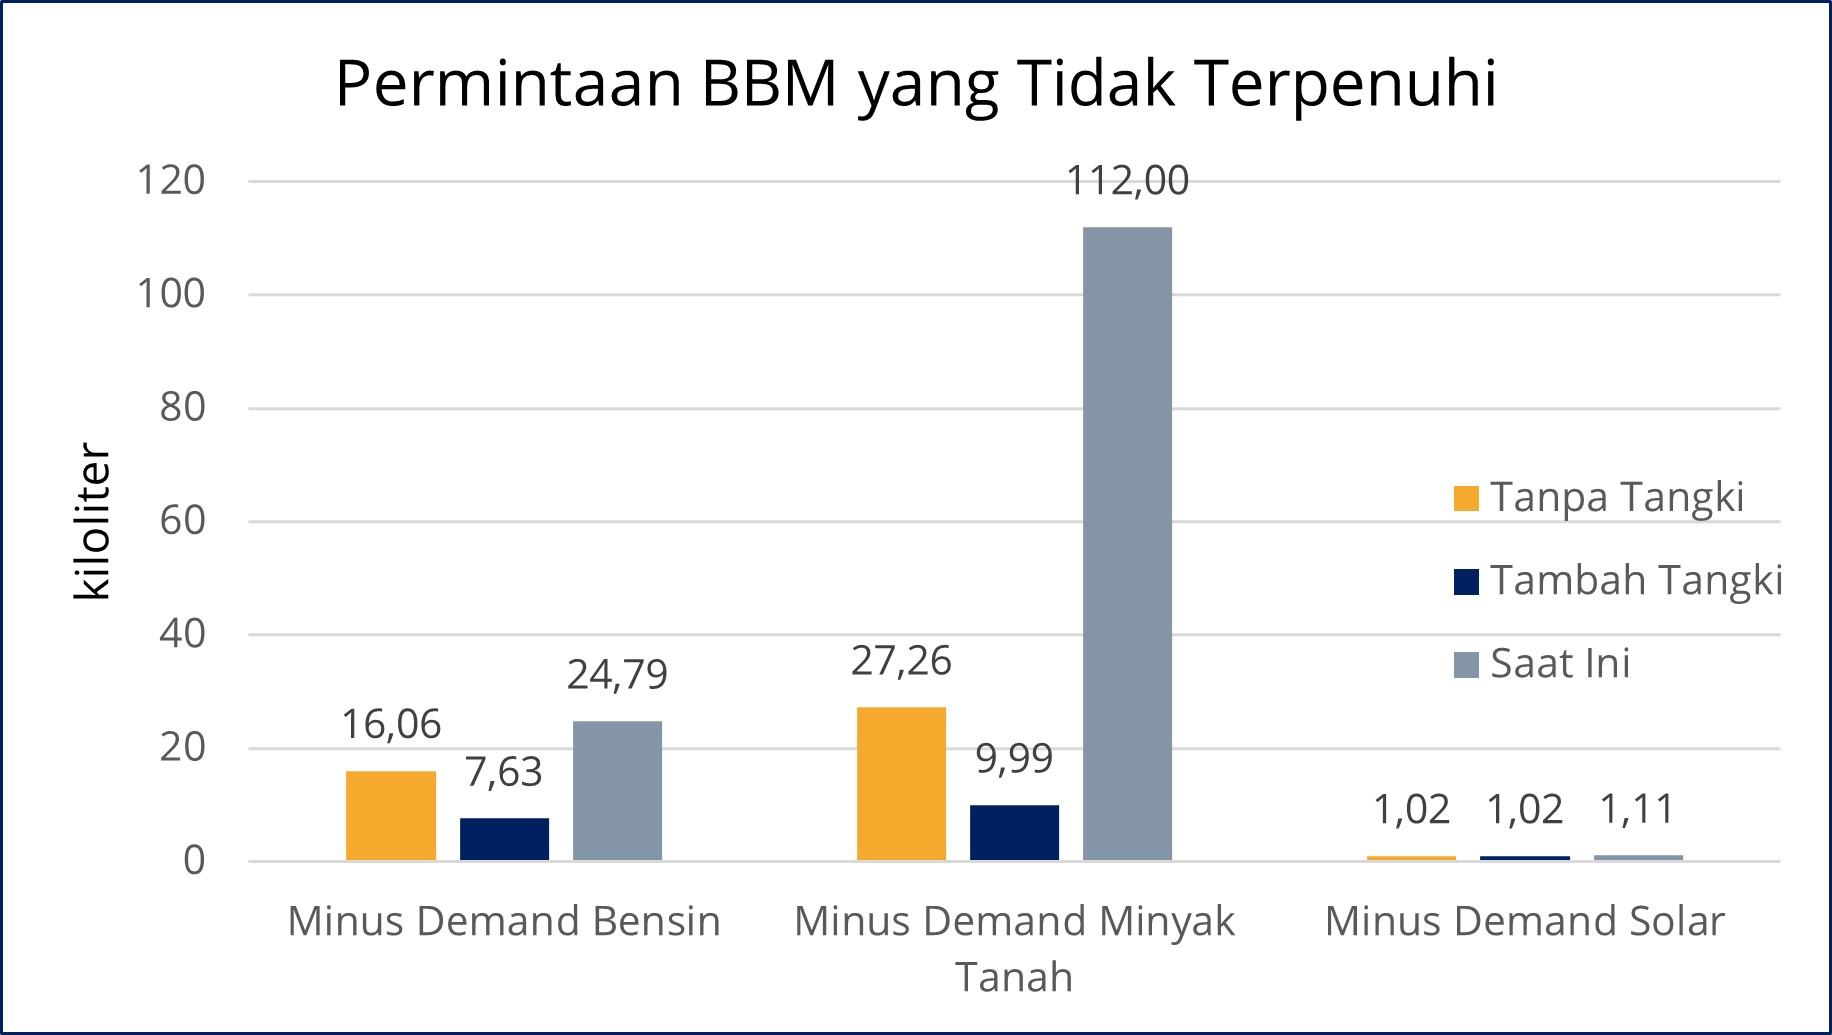
\includegraphics[width=0.75\textwidth]{grafik/minus-bbm-all.jpg}
    \caption{Perbandingan Kelangkaan BBM}
    \label{fig:minus-bbm-all}
\end{figure}

\subsection{Biaya Tahunan}
\label{subsec:total-cost-all}

Biaya masih menjadi konsideran utama untuk mengambil keputusan terutama dalam bidang infrastuktur. Selain biaya tahunan unsur biaya lain yang menjadi pertimbangan dalam perancangan sistem pemasokan BBM ini adalah biaya publik yang mungkin muncul akibat permintaan BBM yang tidak terpenuhi. Biaya publik ini diharapkan mampu memotret keandalan sistem dalam memasok BBM. Sistem pemasokan dengan penambahan tangki menjadi sistem paling optimal dilihat dari rata-rata biaya tahunan dan biaya publik yang muncul, sebagaimana yang terlihat pada gambar \ref{fig:total-cost-all}.

\begin{figure}[!ht]
    \centering
    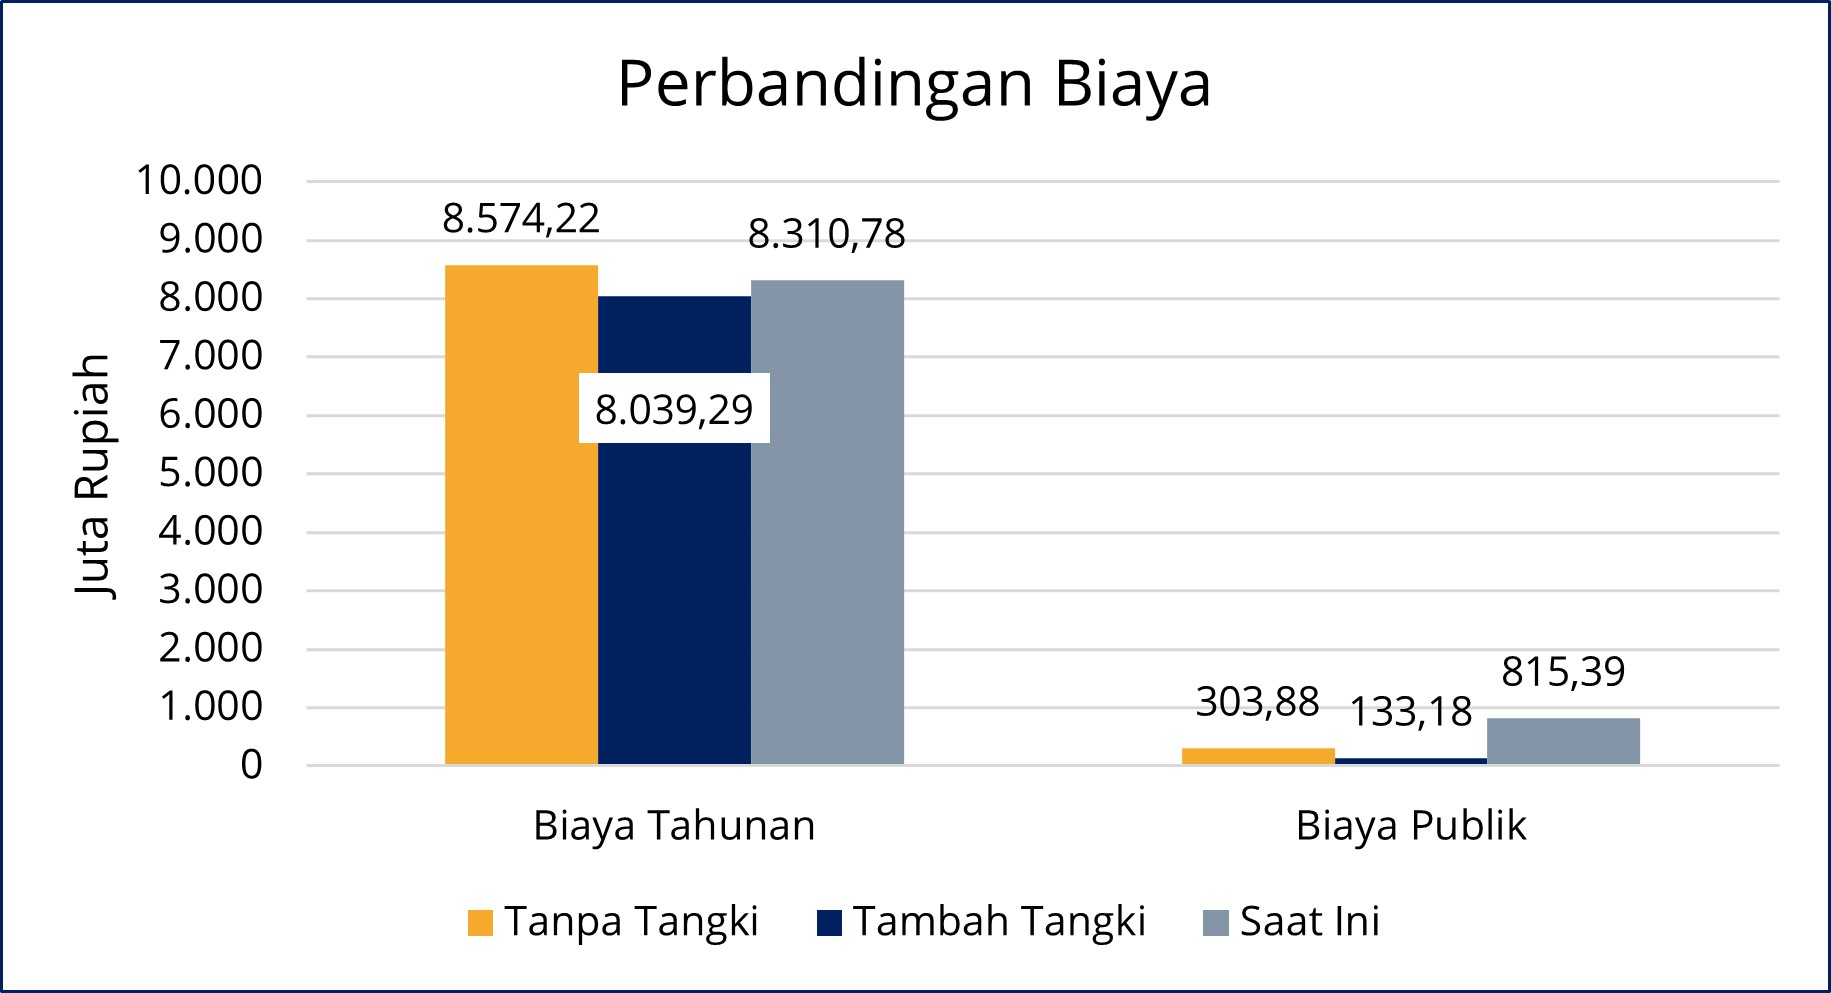
\includegraphics[width=0.75\textwidth]{grafik/total-cost-all.jpg}
    \caption{Perbandingan Biaya Semua Sistem Pemasokan}
    \label{fig:total-cost-all}
\end{figure}

\subsection{Komponen Biaya}
\label{subsec:component-cost-all}

Terdapat perbedaan rasio antara komponen-komponen biaya pada sistem baru. Penambahan tangki memunculkan komponen biaya baru namun mengurangi biaya perjalanan \emph{(voyage cost)} yang muncul. Perbandingan rasio antar komponen biaya dapat dilihat pada gambar \ref{fig:component-cost-all}.

\begin{figure}[!ht]
    \centering
    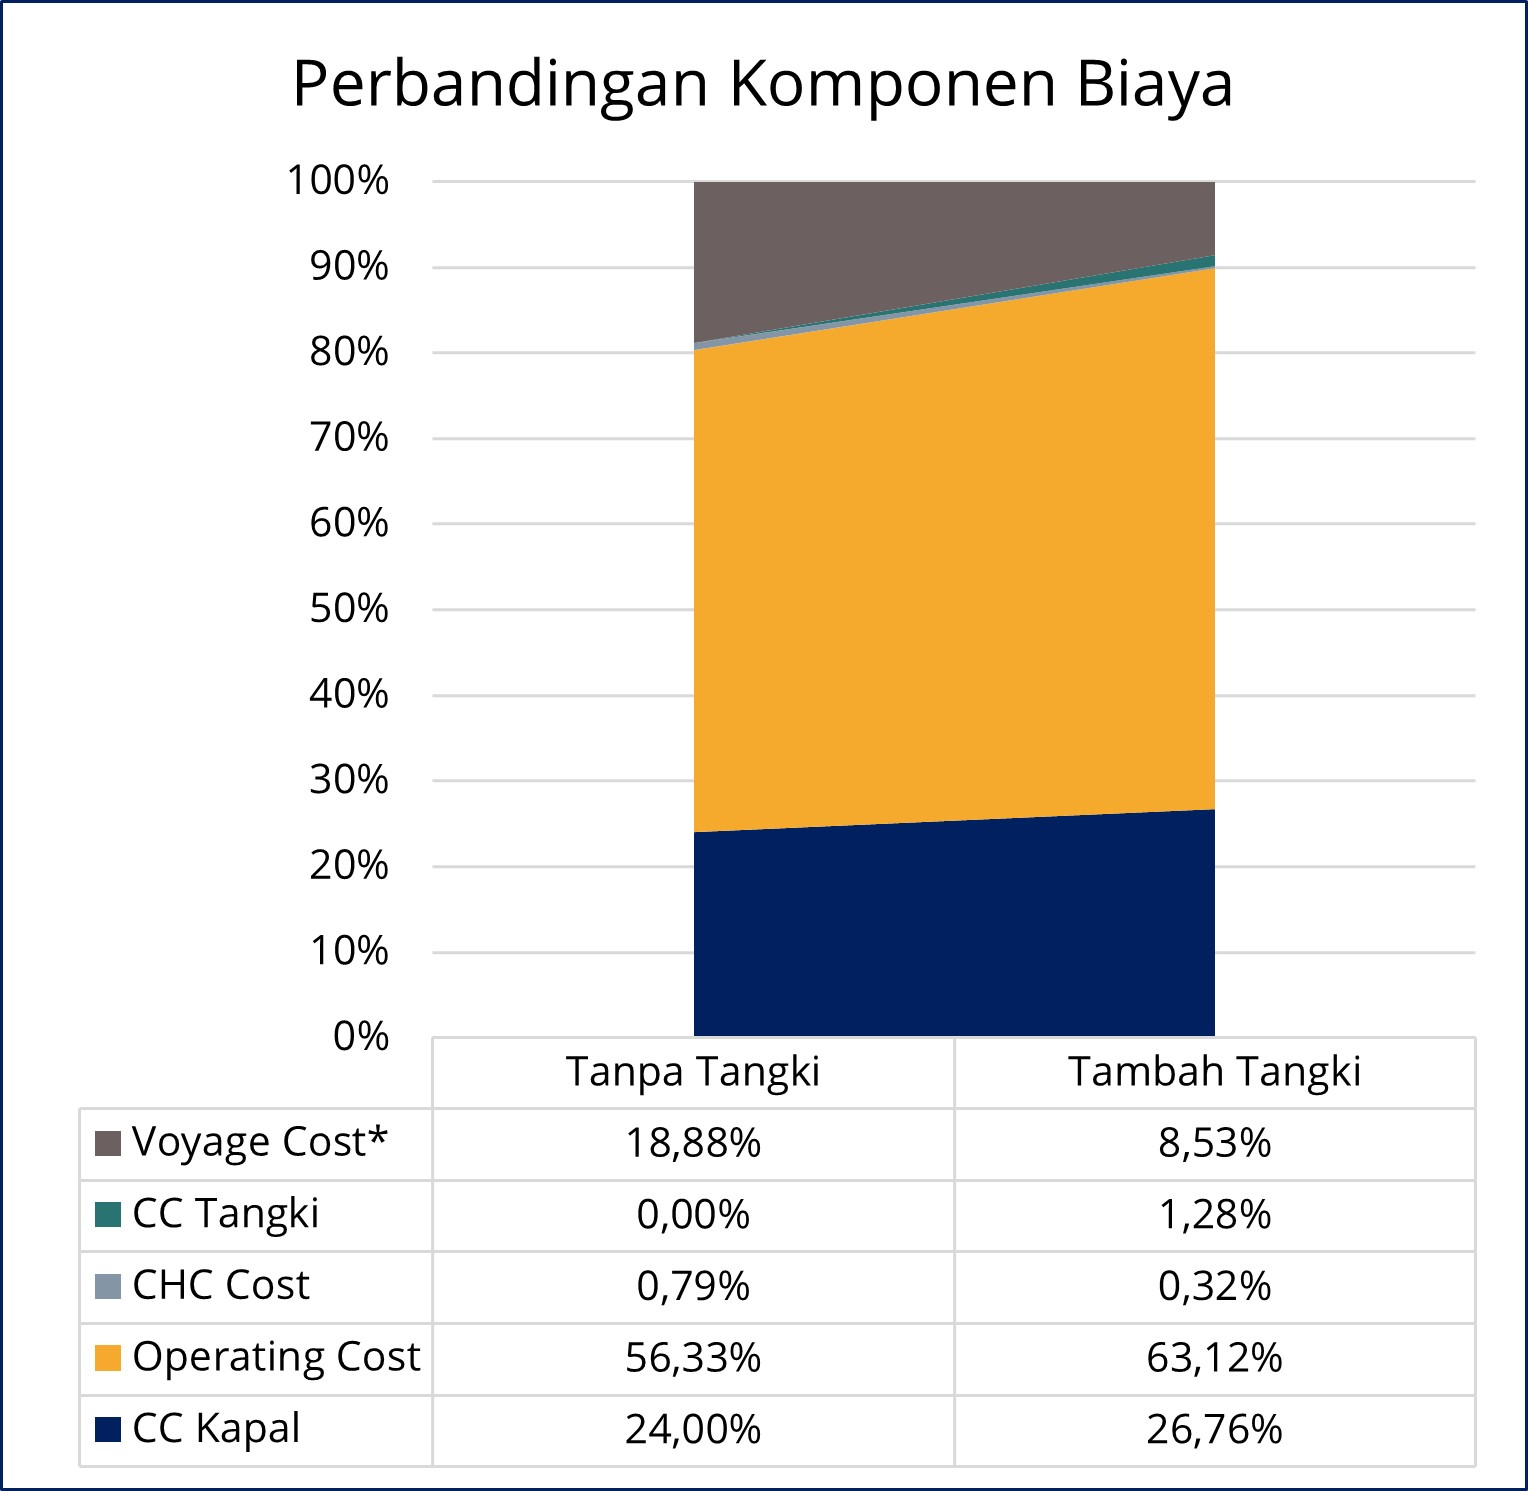
\includegraphics[width=0.75\textwidth]{grafik/element-cost-new.jpg}
    \caption{Perbandingan Komponen Biaya Sistem Baru}
    \label{fig:component-cost-all}
\end{figure}